%
% tests.tex
%
% Copyright (C) 2021 by SpaceLab.
%
% GOLDS-UFSC Documentation
%
% This work is licensed under the Creative Commons Attribution-ShareAlike 4.0
% International License. To view a copy of this license,
% visit http://creativecommons.org/licenses/by-sa/4.0/.
%

%
% \brief Test plan and results.
%
% \author Gabriel Mariano Marcelino <gabriel.mm8@gmail.com>
%
% \institution Universidade Federal de Santa Catarina (UFSC)
%
% \version 0.1.0
%
% \date 2021/01/21
%

\chapter{Test Plan and Results} \label{ch:test-plan}

\section{Test Procedure}

\subsection{Hardware}

.

\subsection{Software}

\subsubsection{Unit Tests}

\begin{itemize}
    \item Hardware checks (might require mock circuitry).
    \item Driver operation checks: not extensive, might use loopback and fake sensor data schemes for hardware checks.
    \item Device operation checks: one test file for each device implemented, more extensive than driver checks, but should avoid development overhead.
    \item Standalone application checks: evaluate the application logic (masking or faking operating system calls, such as waiting for queue or a delay). It should be implement without the operating system, in other words, evaluate inputs/outputs in dedicated main file.
\end{itemize}

\subsubsection{Integration Tests}

\begin{itemize}
    \item Operating system initialization: assert memory allocation (RAM, stack, heap), hooks and etc;
    \item Boot sequence (as similar to the actual procedure as possible).
    \item Operating system task/queue/interrupts priority, constraints, size, depth and delay checks: use dummy task/queue/interrupts (same config as actual system).
    \item Short-term system check: after 1 hour, exit without error logs.
    \item Mid-term system check: after 1 day, exit without error logs.
    \item Long-term system check (used in flatsat): after 1 week, exit without flatsat/integration error logs.
\end{itemize}

\subsubsection{Workflow}

\begin{itemize}
    \item Always it is a build->flash->test, change main and repeat.
    \item It must have a test folder containing subfolders (hardware, drivers, devices, app, integration) and a json file (with name, path and type).
    \item Inside the workflow is called a python script that read this json and setup variables to allow running multiple main file swaps for each test type.
    \item There are 5 different workflows, one for each test type: hardware, drivers, devices, app, integration;
    \item The workflow, tests and scripts must be reviewed before each release.
    \item Idea: for short/mid/long-term tests, the workflow should evaluate the log messages offline instead of real time, in which a job is scheduled to run just after this period and ``a script'' will read the log file and search for the test criteria, giving the actual CI result.
    \item Idea: Inside the code, using the log message approach, we might create our ultra lightweight framework that consists of only log types (colors) and log messages (specific strings). This way we do not modify our current workflow and we can add a simple scheme to access the flight code.
    \item Unit Tests = Tests performed per firmware unit.
    \item Integration Tests = Tests performed per firmware component (several units abstracted).
\end{itemize}

\subsection{Flatsat}

To test all modules during the development of the projet, a flatsat platform was developed. The FlatSat Platform is a testbed for CubeSat PCB modules. FlatSats enable easier, faster and a secure method for testing subsystens independently while been integrated in a flat design before going to integration on a CubeSat form factor. The PCB can support up to 7 modules, all PC-104 pins are interligated to flexibilize its use, only the particularity connection between modules need to be be taken into account. One PC-104 has inverted pinout, the board also makes it possible to have two seperate power supplies, a UART to USB converter for 4 modules, kill-switches activation though SPDTs, Remove Before Flight (RBF) pin header, connector for charging batteries and SMA connectors for antennas. A picture of the flatsat board can be seen in \autoref{fig:flatsat-top}.

\begin{figure}[!ht]
    \begin{center}
        \includegraphics[width=\textwidth]{figures/flatsat_top_image}
        \caption{Top view of the flatsat board.}
        \label{fig:flatsat-top}
    \end{center}
\end{figure}

More information about the Flatsat Platform can be found in \cite{flatsat}.

\subsection{Environmental Tests}

\subsubsection{Mass Verification}

This test checks the total mass of the satellite (without RBF tag), which must be less than 2,66 kg \cite{cds}. The verification is made with a precision balance. \autoref{fig:mass-verification} examplifies this process with FloripaSat-I total mass.

\begin{figure}[!ht]
    \begin{center}
        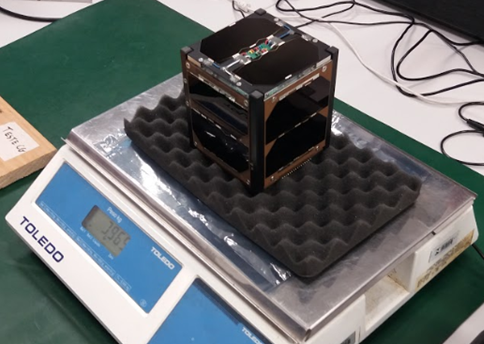
\includegraphics[width=0.5\textwidth]{figures/mass-test}
        \caption{Mass verificatiton of FloripaSat-I.}
        \label{fig:mass-verification}
    \end{center}
\end{figure}

\subsubsection{Center of Gravity}

This test checks the center of gravity (CG) of the satellite, which must be less than 2 cm from the geometric center (see \autoref{fig:cg}) \cite{cds}. To perform this test, a simple test-bench based on two parallel bars fixed on a plate (4 cm from each other) can be used. The geometric center of the satellite is put in the middle of the bars and, if the satellite does not fall, the CG is within the radius of 2 cm. This strategy does not measure the location of CG, however, it does prove if the satellite follows the requirement.

\begin{figure}[!htb]
    \begin{center}
        \subfigure[$X$ axis.\label{fig:fsat-fm-x-axis}]{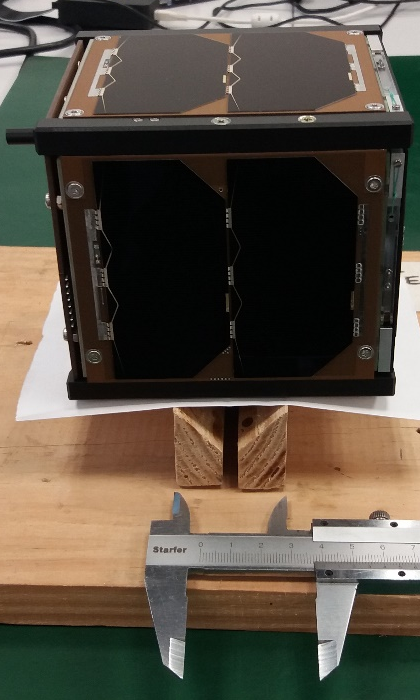
\includegraphics[width=0.2\textwidth]{figures/fsat_fm_x_axis.png}}
        ~
        \subfigure[$Y$ axis.\label{fig:fsat-fm-y-axis}]{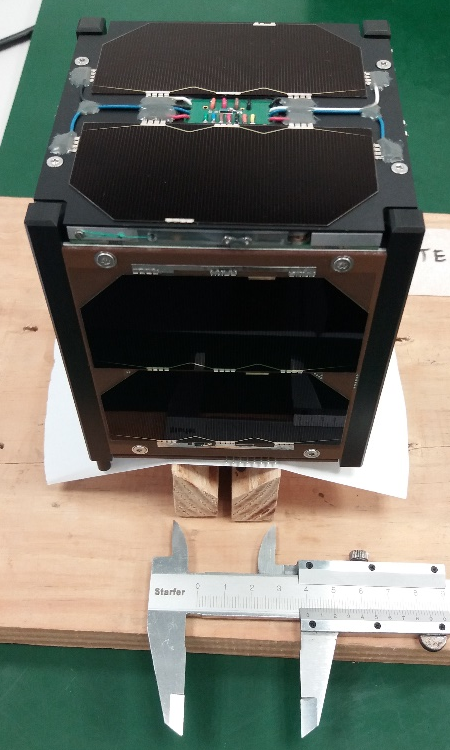
\includegraphics[width=0.2\textwidth]{figures/fsat_fm_y_axis.png}}
        ~
        \subfigure[$Z$ axis.\label{fig:fsat-fm-z-axis}]{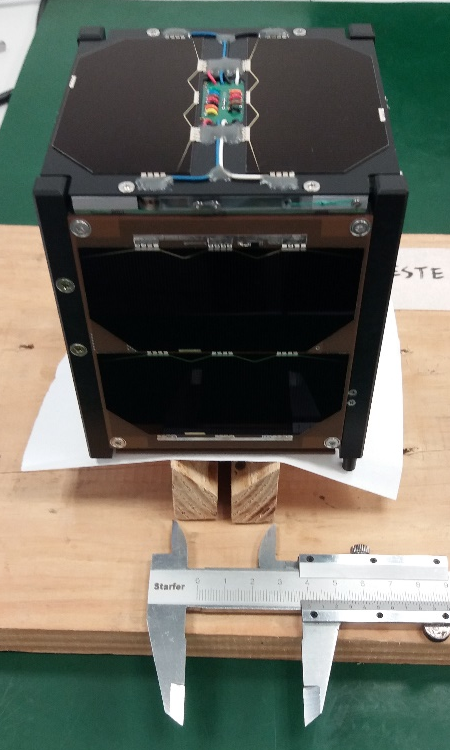
\includegraphics[width=0.2\textwidth]{figures/fsat_fm_z_axis.png}}
        \caption{Center of gravity of FloripaSat-I within 2 cm from geometric center.}
        \label{fig:cg}
    \end{center}
\end{figure}

\section{Preliminary Results}

.
